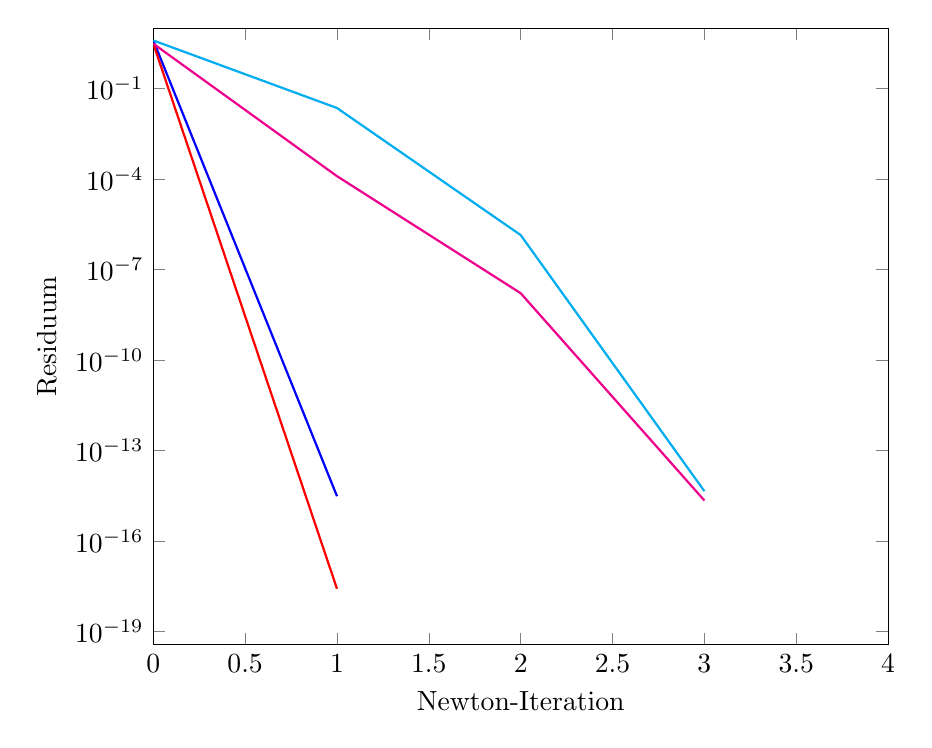
\begin{tikzpicture}[every plot/.append style={thick}] 
\begin{axis}[ 
label style={font=\normalsize}, 
xlabel={Newton-Iteration}, 
ylabel={Residuum}, 
xmin=0, xmax=4, 
ymode=log, 
ymin=0, ymax=10, 
width=0.9\textwidth, 
grid style=dashed, 
] 
\addplot[ 
color=blue, 
] 
coordinates { 
(0, 3.94e+00)(1, 3.02e-15)}; 
\addplot[ 
color=red, 
] 
coordinates { 
(0, 3.07e+00)(1, 2.57e-18)}; 
\addplot[ 
color=cyan, 
] 
coordinates { 
(0, 3.94e+00)(1, 2.26e-02)(2, 1.38e-06)(3, 4.45e-15)}; 
\addplot[ 
color=magenta, 
] 
coordinates { 
(0, 3.07e+00)(1, 1.24e-04)(2, 1.63e-08)(3, 2.18e-15)}; 
\end{axis} 
\end{tikzpicture} 
